%!TEX root = comps_NKasimov.tex
\chapter{Introduction}
\label{chapter:1}

\section{Motivation and Objective}
This project is supported by ONR MURI on Soil Blast Modeling. It is a part of a bigger multiscale/multiphysics project on research and simulations of explosions of buried explosive devices~\cite{proc:muri}. In Figure~\ref{fig:muri_motiv} one can see ejecta under asphalt pavement after improvised explosive device (IED) explosion hitting U.S. military convoy, which is starting point of the project. Main motivation of the project is overcome wide variety of uncertainties that occur at the moment of explosion (blast wave propagation) due to the soil type, moisture, density; landmark peculiarities, explosive type, and etc., so one can better predict harmful effect of the explosion and perform a proper defensive strategies such as armoring.
\begin{figure}[h!]
\centering 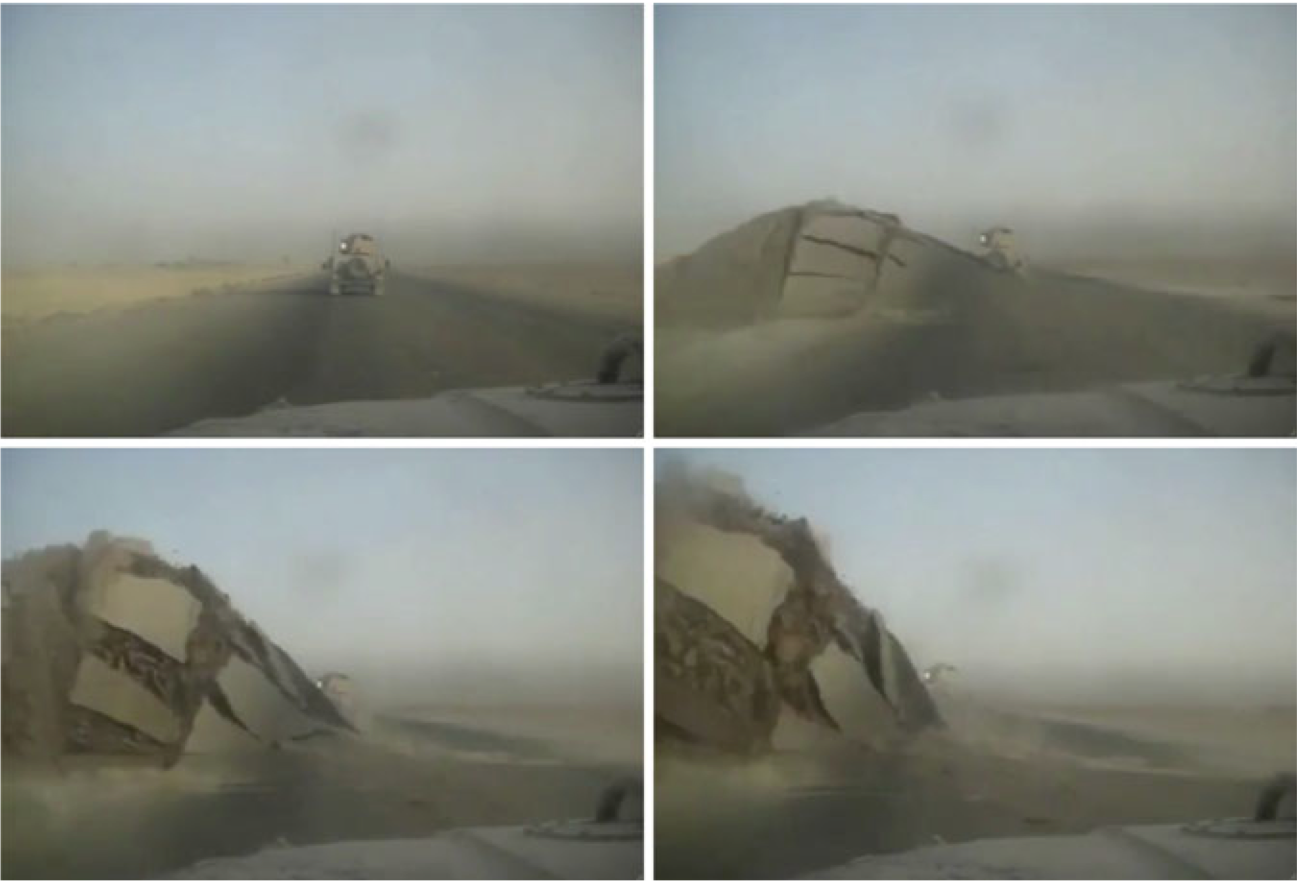
\includegraphics[scale=0.25]{fig/muri_motiv.png}
\caption{IED explosion in Iraq, hitting U.S. military convoy} \label{fig:muri_motiv}
\end{figure}

Existing methodologies allow to do simulations on each peculiarity consisting this complex phenomenon separately but not for all of them simultaneously using coupled equations. The main focus of this project is to provide a low fidelity computation model of fluid-structure interaction of compressible supersonic flow around multiple solid particles. The model is based on high fidelity DNS simulations involving several orders of magnitude less number of particles and properly extrapolated and/or averaged in order to couple with other approaches. For that purpose new volume penalization method is developed for high fidelity simulations \cite{ebd_nk_ovv_cbvp_jcp}. For low fidelity simulations volume penalization method roughly based on Brinkman method is developed, which mimicked boundary conditions on fluid-particle interface but which also took into the account extremely rough grid, i.e. boundary layer is not resolved.
\section{Methodology}
In this project several numerical techniques are used to address different parts of the framework. High fidelity simulations utilized Characteristic Based Volume Penalization (CBVP) method developed by O.~V.~Vasilyev, E.~Brown-Dymkoski and N.~Kasimov. To address discontinuities in flow parameters (shock waves) specific artificial viscosity method based on wavelets is used \cite{lib:RegVas}. Local grid refinement (data compression) and corresponding differentiation on adaptive grid is achieved using Adaptive Wavelet Collocation Method (AWCM) \cite{lib:wlt_main}. Low fidelity simulations are performed using Briknman-like momentum penalization of Euler equations (inviscid flow) in order to match drag force. Riemann solver of Roe is used as a shock capturing scheme \cite{book:Toro}. Particle-particle interaction is calculated using DEM/FEM method and later coupled with CFD part of the solver.
\subsection{Volume penalization}
In order to handle flows around solid obstacles numerically, several approaches are used. One can classify them into two main categories --- Body Fitted Grid (BFG) methods and Immersed Boundary methods (IB) \cite{lib:ib_peskin}. BFG methods allow to construct typically curvilinear grid in such a way that obstacle boundary is aligned with grid lines (See Figure.~\ref{fig:radial2rect}a), so no special treatment of the boundary conditions at the obstacle is needed.
\begin{figure}[h]
\begin{minipage}{0.5\linewidth}
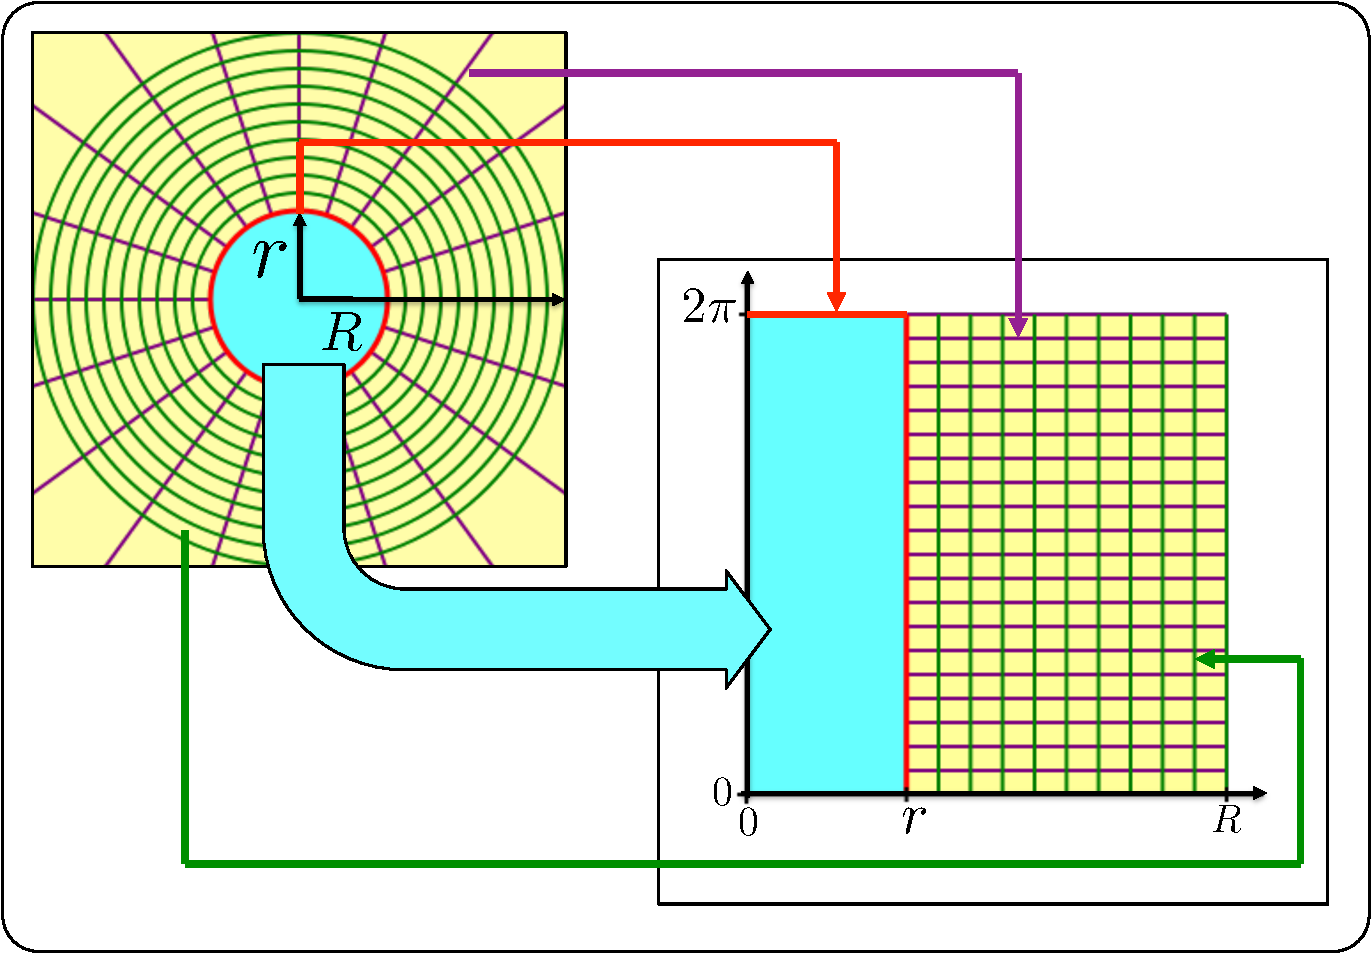
\includegraphics[width=\linewidth]{fig/radial2rect.pdf}
a) Circlualr object and grid lines \label{fig:radial2rect_a}
\end{minipage}
\begin{minipage}{0.5\linewidth}
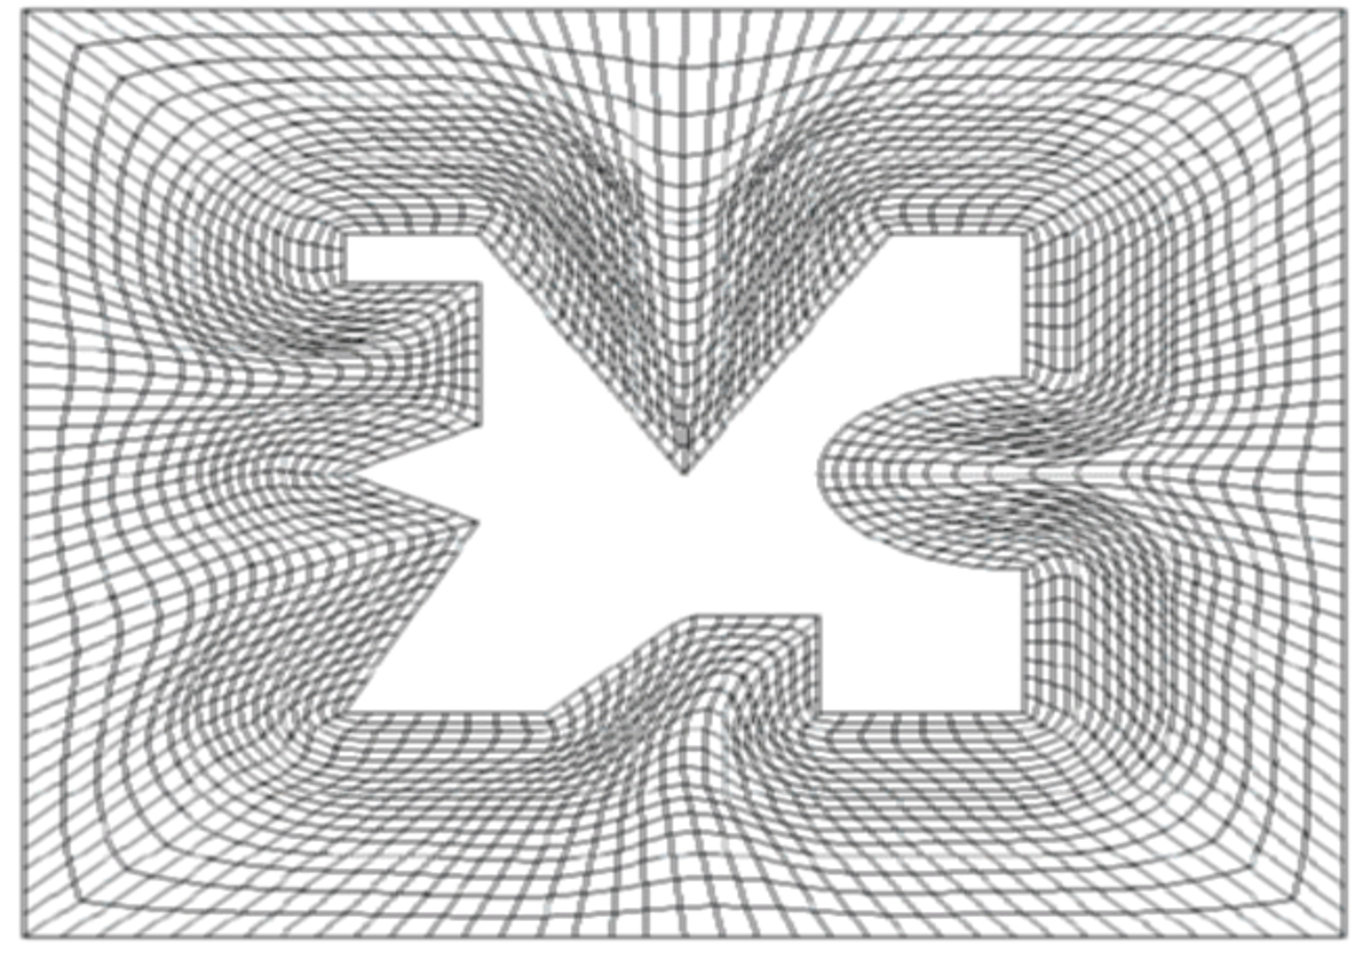
\includegraphics[width=\linewidth]{fig/weird_shape.pdf}
\centering b) More complex shape \label{fig:radial2rect_b}
\end{minipage}
\caption{Body fitted grid examples} \label{fig:radial2rect}
\end{figure}\\
In order to get rectilinear system as in Figure~\ref{fig:radial2rect}(a) one need to perform radial transformation
\begin{align*}
x &= x_0 + r\cos \varphi \\
y &= y_0 + r\sin \varphi
\end{align*}
and change all equations accordingly. In most cases obstacles have more complex shapes (see Figure~\ref{fig:radial2rect}b) and finding corresponding transformation of the coordinates might be problematic. Additional difficulties arise when obstacle is allowed to move and deform due to the interaction with the flow --- new transformation should be found at each time step.

IB methods, Volume Penalization (VP) methods in particular, in contrary, do not change existing grid, but rather change governing equations, i.e. they are intrusive methods. Equations are modified through artificial forcing terms that are added to the governing equations so that solution at the boundary tends to the exact solution. The methodology underlying this project is a VPM.
\subsubsection{Brinkman Penalization Method}
\label{sec:brinkman_penal_chapter1}
The first VPM that is used at early stage of the project is Brinkman Penalization method (BPM), originally proposed by Arquis and Caltagirone \cite{lib:vp_brink} for incompressible flow around solid obstacles through momentum penalization. This method is successfully extended to the subsonic compressible flow~\cite{lib:vp_liu}. The main advantages of the method are systematic error control and relative simplicity of numerical implementation. The very basic interpretation of the method can be achieved if one represents solid obstacle as a porous media with controlled permeability and porosity.

\subsubsection{Characteristic Based Volume Penalization}
BPM applied ``as it is'' to supersonic flows led to numerous errors, such as inaccurate acoustic reflection, pressure seepage, phase lag, etc. Also the fact that BPM cannot be used to model boundary conditions other than Dirichlet and homogeneous Neuman made it difficult for some type of simulations with Neumann and Robin type boundary conditions. In order to handle these deficiencies new VPM is developed --- Characteristic Based Volume Penalization. To mimic Dirichlet type boundary conditions CBVP still utilizes BP with some modifications to enhance numerical stability. For Neumann and Robin type boundary conditions the solution is propagated inside of the obstacle along inward directed normal vector, hence the name of the method. 

\subsubsection{Brikman-like Volume Penalization, Low Fidelity Simulations}
For Low Fidelity simulations supersonic flow is modeled using extremely coarse grid. The latter restricted us to resolve boundary layer, so Euler equation are used instead. To mimic drag force caused by the flow as in case of the viscous flow, we introduced penalization of the momentum equation. Also, due to the coarse grid, in case of many obstacles amount of the flow penetrating the obstacle could lead to significant numerical errors. To fix it, another penalization terms related to the porosity is introduced, which is also inspired by BPM.

\subsection{Adaptive Wavelet Collocation Method}
In order to achieve data compression, i.e. to use fewer grid points than if one utilizes uniform rectangular grid, AWCM is used. The main advantage of the method is systematic a priori error control while maintaining structured rectilinear grid. Second generation interpolation wavelets are used as basis functions. Grid adaptation algorithm underlying the method allows to both accurately track regions of ``important physics'' and easily program it using existing numerical platforms. Tracking can be performed for dynamically changing phenomena without significant overhead --- in many cases extra calculations are overcompensated by high data compression.

\subsection{Shock Capturing Scheme}
To handle discontinuities in High Fidelity simulations, shock capturing scheme based on AWCM is used. It is based on the solution of hyperbolic equation near the discontinuities/shocks in order to smooth them with desired width. This procedure introduces non-linear artificial viscosity. The main reason to incorporate this method with AWCM is that latter serves as a good indicator of shock location through wavelet coefficients. Method exhibits good localization property, avoiding unnecessary smoothing in the regions where it is not required. 

\subsection{Shock Capturing Scheme, Low Fidelity Simulations}
To handle discontinuities in Low Fidelity simulations Riemann solver of Roe is used. This method is equivalent to using artificial viscosity, although it cannot be controlled and viscosity value is defined by the flow. Main procedure underlying the method is performing certain type of averaging of flow parameters, so called Roe average. After the averaging, Euler equations become pseudo linear hyperbolic equations. Roe solver handles transonic and subsonic regions of the solution worse than discontinuities, although there are ways to overcome this issue, such as so called Harten-Hyman Entropy Fix.

\subsection{CFD/DEM Coupling, Low Fidelity Simulations}
In Low Fidelity simulations, due to the coarse CFD grid, it is possible to model supersonic flow around large number of particles that might interact with both flow and other particles. CFD-DEM coupling provides particle-particle and fluid-particle interactions, while CBVP provides particle-fluid interactions, closing the system. The only restriction applied to the system is to have same global time step for both CFD and DEM solvers, which in some cases might be inefficient. 


\section{Organization}
The rest of this paper is organized as follows. In Chapter 2, the necessary background of Volume Penalization techniques, shock capturing schemes, Adaptive Wavelet transforms and basics of CFD-DEM coupling will be covered. Testing different numerical techniques with proper algorithm justification of chosen or developed algorithms is discusses in Chapter 3. In Chapters 4 and 5 one can find results of High Fidelity and Low Fidelity simulations accordingly. Future work is presented in Chapter 6.
